\chapter{Design}
\label{chap:design}

Design by mohl být definován jako aktivita, jejíž úkol je přenést nápad, představu nebo myšlenku něčeho užitečného do zpracovatelné podoby, ať už se jedná o auto, budovu, službu nebo proces. Jde o množinu činností, jež má za úkol pomoct lidem v orientaci a učinit jejich život jednodušší. Design je součástí každodenního života, ať už se nacházíme uvnitř budovy, na autobusovém nástupišti nebo procházíme Internetové stránky---může se jednat o model auta, interiér budovy nebo informační systém; představuje způsob jak věci vypadají, jak fungují a jak moc pozornosti přitahují nebo nepřitahují. Existují samozřejmě případy, kdy je nežádoucí, aby design přitahoval příliš mnoho pozornosti. Úkolem designera je tedy vžít se do role uživatele, do jeho chování a potřeb. Pouze designeři mohou proměnit koncept v něco žádoucího, hodnotného a komerčně úspěšného.

Již ve 2. polovině 20. století se zrodil zcela nový obor anglicky nazvaný \textit{computer science}. Tento obor dnes označujeme jako informatika. Informatika má zásadní vliv na design a to nejen na samotný proces tvorby---díky informačním technologiím vznikly zcela nové oblasti designu. Každá aplikace, služba nebo statická webová stránka potřebuje rozhraní, které bude sloužit jako vrstva komunikující s uživateli.

Při vzniku prvních operačních systémů vznikla snaha vývojářů a designerů unifikovat grafické uživatelské rozhraní. Tento druh unifikace měl za úkol poskytovat uživatelům intuitivní prostředí a tím zredukovat nutnost porozumět všem různým variacím uživatelských rozhraní grafických aplikací. S rozšířením Internetu se toto úsilí přenáší především na designéra a společnost je tak vystavena daleko většímu množství nových grafických rozhraní a technologií. Tento trend je zodpovědný za vznik mnoha nových pojmů a konvencí.

Mezi designery se v posledních letech rozšířilo několik nových termínů, které mají za úkol jednoznačně rozlišit jednotlivé činnosti a profily webdesignu. Podstatou těchto pojmů je zároveň usnadnění komunikace mezi designéry, mezi ty nejpodstatnější patří---

\begin{itemize}
    \item Použitelnost (Usability)
    \item UI (User Interface)
    \item UX (User eXperience)
\end{itemize}

Tyto pojmy se navzájem prolínají, jejichž primárním cílem je specifikace zásad a doporučení pro úspěšné dokončení tvorby uživatelského rozhraní.

V rámci vysvětlení těchto pojmů budu používat termín \uv{produkt}, který může představovat aplikaci, elektronické zařízení, nebo službu.

\section{Použitelnost}
\label{sec:usability}

Použitelnost je soulad užitečnosti a jednoduchosti použití. Produkt je použitelný pokud:

\begin{itemize}
    \item je pro uživatele užitečný a vyhovuje jeho potřebám;
    \item je jednoduché naučit se produkt používat;
    \item je efektivní produkt používat---zabere málo času vykonat nějaký úkol;
    \item je produkt málo náchylný na chyby.
\end{itemize}

Dobře použitelný produkt musí do jisté míry splňovat všechny tyto body. Existuje mnoho produktů, které jsou natolik složité, že většinu uživatelů odradí od normálního používání (pokud ovšem mají možnost volby). Často se přitom jedná o vysoce užitečné a produktivní aplikace---typickým příkladem jsou informační systémy, které obsahují ohromné množství dat a nástrojů se kterými musí uživatelé manipulovat.

Mezi některé typické příklady špatné použitelnosti u webových aplikací patří například absence vyhledávače, nutnost registrace pro zobrazení většiny obsahu nebo dlouhé registrační formuláře a nečitelná CAPTCHA\footnotemark[1]. Použitelnost lze přitom snadno zvýšit dodržováním určitých zvyklostí. Jako jedna z důležitých vlastností dobře použitelných aplikací je často označována typografie (viz \ref{sec:typografie}), jejíž správné provedení však vyžaduje hlubší znalosti.

\footnotetext[1]{Akronym pro \textit{Completely Automated Public Turing test to tell Computers and Humans Apart}, jedná se o techniku určenou pro odlišení skutečného uživatele od (Turingova) stroje.}

\section{UI design}
\label{sec:uidesign}

UI design zahrnuje práci designerů, kteří vytvářejí hmatatelné prvky se kterými uživatele pracují. UI designeři se soustředí na vizuální podobu a použitelnost produktu. Použitelnost je tedy nutnou součástí kvalitních uživatelských rozhraní.

Uživatelské rozhraní webových aplikací prošlo v posledních letech zásadním vývojem---za tento vývoj je zodpovědná především rozšířenost webových technologií (HTML, CSS a JavaScript) a s tím související popularita majoritních webových prohlížečů. Ještě nedávno patřil mezi nejpopulárnější prohlížeče Internet Explorer, který má dodnes nejhorší podporu moderních webových technologií. S tím, jak jsou protlačovány nové technologie, se zvyšuje \uv{svoboda} designérů a kodérů, kteří nejsou omezováni schopnostmi postarších prohlížečů.

\section{UX design}
\label{sec:uxdesign}

UI design je část produktu, se kterou přichází uživatel do kontaktu, když se na produkt podívá. UX design je pocit nebo dojem, který produkt vyvolává, když jej uživatel používá \cite{ui-vs-ux}. UI design je nutnou součástí UX designu, stejně jako je použitelnost součástí UI designu (viz obrázek \ref{fig:ux-ui-usability}).

\begin{figure}[htbp]
    \centering
    \includegraphics[width=10cm]{images/ux.pdf}
    \caption{Podíl UX, UI a použitelnosti v designu.}
    \label{fig:ux-ui-usability}
\end{figure}

Příklady některých vlastností a kvalit, které mají vliv na dobrý UX design webových aplikací:

\begin{itemize}
    \item \textbf{Obsah}. Kvalita obsahu, struktura textu, obrázků a dalších typografických prvků.
    \item \textbf{Výkon}. Rychlost aplikace a její dostupnost.
    \item \textbf{Diskuze}. Podpora diskuzí, hodnocení produktů.
    \item \textbf{Způsob platby}. Příležitost internetové platby (platba kartou, PayPal apod.)
    \item \textbf{Reklama}. Výskyt reklam a jejich způsob zobrazení \cite{understanding-ux-ui}.
\end{itemize}

\section{Typografie}
\label{sec:typografie}

\begin{quote}
    \uv{Typografie je organizace písma v ploše} \cite{svalbach}
\end{quote}

\noindent
Typografie je ještě starší než samotný design, její počátky sahají do 15. století, kdy Johannes Gutenberg vynalezl knihtisk. Už tehdy si typografové uvědomovali její důležitost. Během nadcházejících století se typografie rozšířila do novin, informačních systémů a reklam. Popularita typografie měla za následek rozvoj mnoha rodin písma, jejichž elektronické modifikace se používají i u dnešních zařízení.

Webdesign je z 95\% typografie---toto tvrzení vyplývá ze skutečnosti, že 95\% informací na internetu se nachází v písemné podobě \cite{typography}. Typografie je zásadním prvkem pro tvorbu webových aplikací, jedná se o primární způsob přenosu informací mezi aplikací a uživatelem. Tento fakt klade určité nároky na kvalitní uživatelské rozhraní. Knižní typografie prošla dlouholetou evolucí a pokrokem, je tedy inspirací pro kvalitní typografii na webu.

\subsection{Volba čitelných fontů}

Pro nadpisy a podnadpisy je doporučeno používat patkové písmo, neboť je čitelnější, naopak pro text vysázený nižší velikostí písmem bezpatkové. Toto doporučení vychází ze skutečnosti, že displeje s nízkým PPI (počtem pixelů na palec) radikálně snižují čitelnost patkových fontů.

\subsection{Šířka odstavců}

Příliš dlouhé řádky textu snižují koncentraci čtenáře---tento jev je dán nezbytností získat představu o tom, kde řádek končí a kde nový začíná. Naopak krátké řádky nutí návštěvníka číst příliš přerušovaně. Délka odstavce by měla odpovídat přibližně 55--90 znakům na řádek.

\subsection{Velikost písma}

Minimální doporučovaná velikost písma je 16$px$, což je přibližně stejná velikost, jako velikost textu vytištěného v knize nebo magazínu \cite{min-font-size}.

\subsection{Velikost okrajů}

Okraje oddělují důležitý obsahu od méně významných částí webu a dovolují čtenáři soustředit se na text. Doporučený poměr okrajů na webu je 2~\textbf{:}~3~\textbf{:}~4~\textbf{:}~3\footnotemark[1], velikost okrajů pak 2$em$~\textbf{:}~3$em$~\textbf{:}~4$em$~\textbf{:}~3$em$, kde 1$em$ je roven dvojnásobku velikosti fontu.

\footnotetext[1]{V poměru \textit{vrchní strana} \textbf{:} \textit{pravá strana} \textbf{:} \textit{spodní strana} \textbf{:} \textit{levá strana}.}

\subsection{Řádkování}

Podobně jako šířka odstavců i řádkování ovlivňuje nutnost koncentrace čtenáře. Minimální doporučené řádkování je 1.3$em$, je však závislé na střední výšce použitého fontu.

\subsection{Kontrast textu}

Kontrast má velký vliv na čitelnost, nízký kontrast zvyšuje únavu očí, naopak příliš vysoký kontrast působí dráždivě \cite{eye-strain}. Jedna z doporučených kombinací je tmavě šedý text na bílém podkladu.

\begin{figure}[htbp]
    \centering
    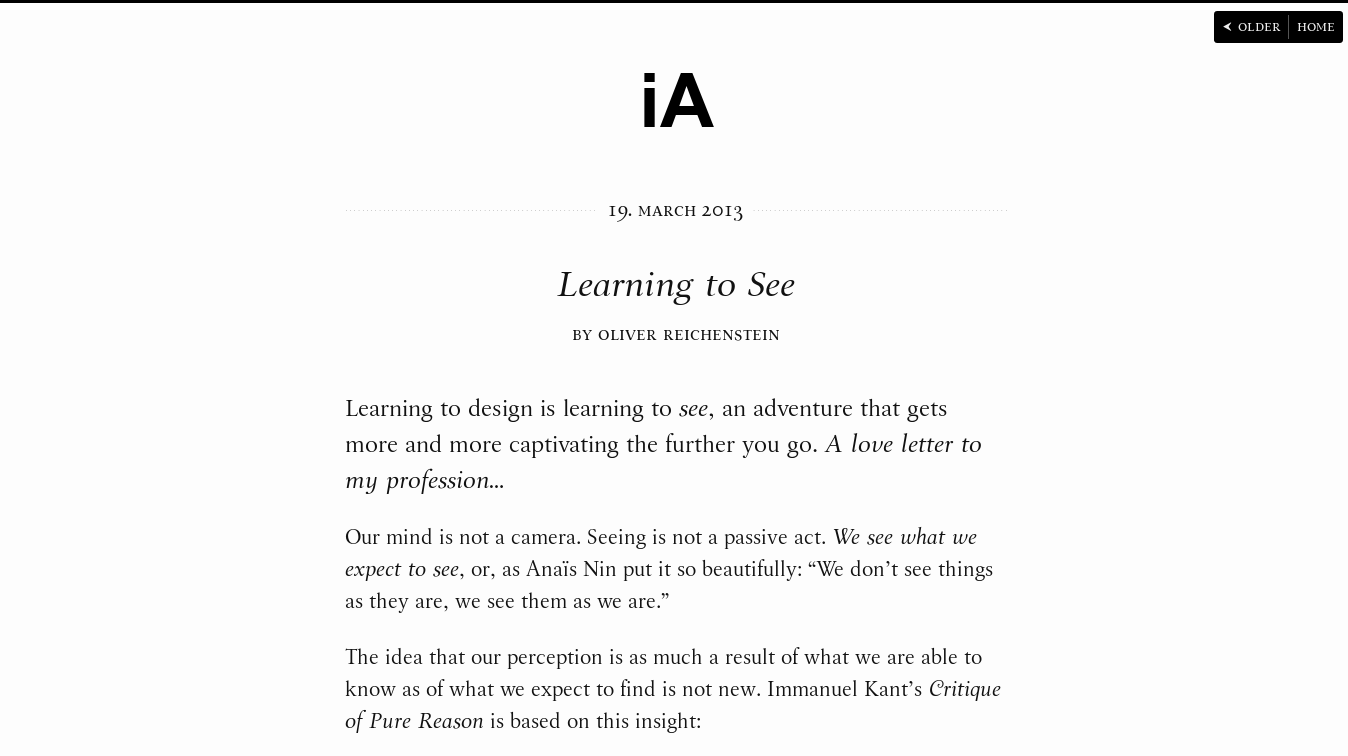
\includegraphics[width=\textwidth]{images/typography.png}
    \caption{Příklad webové stránky, kde autor použil výhradně typografické prvky. Na stránce si můžeme všimnout použití pouze jedné rodiny písma. Zdroj: \url{http://informationarchitects.net/}.}
    \label{fig:web-typography}
\end{figure}
